\section{L'erreur comme source de la connaissance scientifique}
\begin{myepigraph}
\og{}Les vraies révolutions sont lentes et elles ne sont jamais sanglantes\fg{}\\[-1ex]
\normalfont{--- \citet{anouilh1956pauvre}}\\ 
\end{myepigraph}
\medskip
La science progresse en corrigeant constamment les erreurs, c'est-à-dire que les erreurs précèdent nécessairement l'établissement de la connaissance scientifique. Bien que ce processus de correction des erreurs puisse être observé de manière diachronique, il est de nature circulaire. En outre, si une doctrine devient obsolète avec le temps et l'avènement des technologies avancées permettant de recueillir de nouvelles preuves, une doctrine actuellement en vigueur deviendra tout de même à son tour obsolète à un moment\footnote{L'un des exemples le plus connu de l'obsolescence scientifique est sans doute le passage du modèle géocentrique de l'univers, défendu par Aristote et Ptolémée (selon lesquels la Terre est immobile au centre de l'Univers), à la conception héliocentrique de Nicolas Copernic, qui affirmait que la Terre tournait autour du Soleil.}.
\begin{figure}[h!]
    \centering
    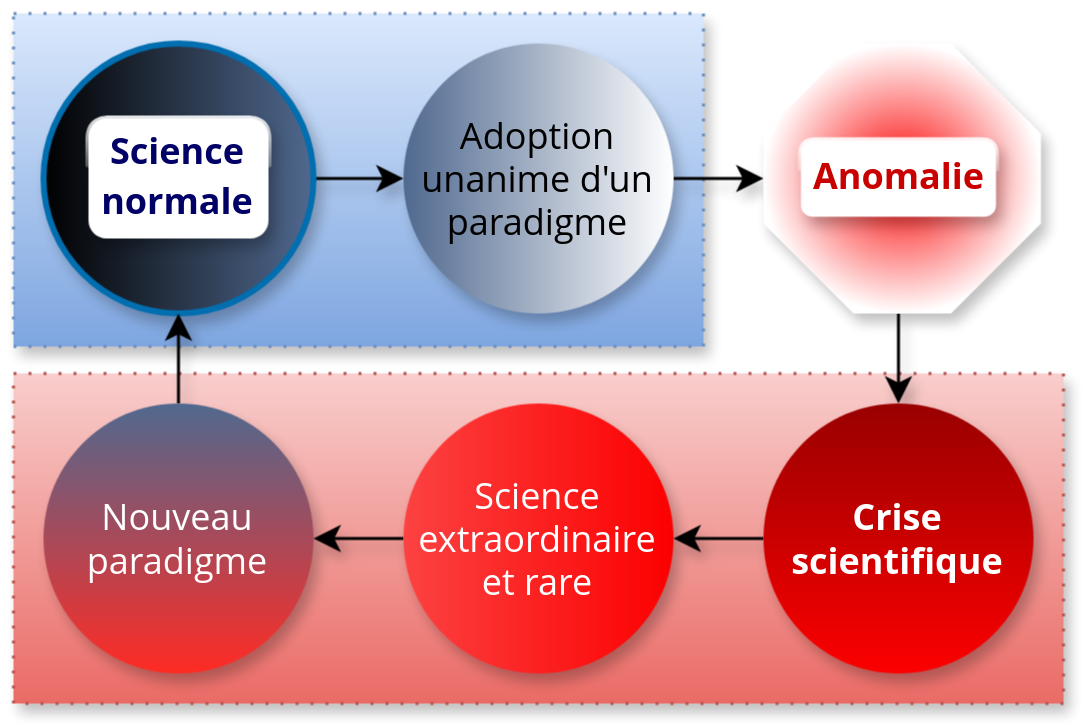
\includegraphics[width=75mm,scale=0.5]{img/changement_paradigme.png}
    \caption{Conception kuhnienne du progrès scientifique, adaptée de \citet{amiri2012}.}
    \label{fig:enter-label}
\end{figure}
%\textit{doxa} (croyance)\footnote{Du grec ancien \textgreek{δόξα} signifiant \og{}opinion\fg{}.} d'hier devient \textit{épistémè} (connaissance)\footnote{Du grec ancien \textgreek{ἐπιστήμη} signifiant \og{}science\fg{}.} d'aujourd'hui, le dernier terme devenant à son tour doxa du lendemain, à la lumière de nouvelles preuves, et ainsi de suite\footnote{Dans \textit{République}, \textit{478}c, Platon oppose la \og{}croyance philosophique, doctrine\fg{} (\textgreek{δόξα}) à la \og{}science\fg{} (\textgreek{ἐπιστήμη}).}. 

Un tel cycle des observations empiriques peut être bouleversé, selon \citet[p. 26]{bachelard1934formation}, par la \og{}rupture et non pas continuité entre l'observation et l'expérimentation\fg{}. Autrement dit, la rupture épistémologique survient lors d'un renversement fondamental dans la façon d'établir une connaissance dans un domaine particulier. De fait, ce phénomène caractérise une \og{}révolution scientifique\fg{} \citep{koyre1957closed}, terme apparenté avec celui du \og{}changement de paradigme\fg{}, introduit par \citet{kuhn1962structure}. D'après ce dernier, les \textit{paradigmes} désignent les \og{}découvertes scientifiques universellement reconnues qui, pour un temps, fournissent à une communauté de chercheur$\cdot$euse$\cdot$x$\cdot$s des problèmes types et des solutions\fg{}. 

Dans cette optique$\dots$ (continuer depuis ici)

%Un tel cycle des observations empiriques représente, selon \citet{koyre1962monde}, une \og{}révolution scientifique\fg{}, terme apparenté avec celui du \og{}changement de paradigme\fg{}, introduit par \citet{kuhn1983structure}. Dans cette optique, la structure des révolutions scientifiques désigne un modèle épistémique constitué des épisodes non cumulatifs de développement. Le nouveau paradigme ne désigne pas une extension de l'ancien paradigme ; au contraire, le dernier est entièrement ou partiellement remplacé par un nouveau paradigme incompatible avec le précédent, ce qui montre que le développement historique des théories est discontinu.
%
%Dans un esprit similaire, ce point épistémologique est relevé par \citet{bachelard1970idealisme} qui souligne :

\begin{quote} 

\og{}Il ne saurait y avoir de vérité \textit{première}. Il n'y a que des erreurs \textit{premières.}  [...]. La première et la plus essentielle fonction de l'activité du sujet est de se tromper. Plus complexe sera son erreur, plus riche sera son expérience. L'expérience est très précisément le souvenir des erreurs rectifiées. L'être pur est l'être détrompé. \fg{} 
%\flushright{\cite{bachelard1970idealisme}} 
% \flushright{\cite[p.~89]{bachelard1970idealisme}} 

\end{quote}

Un exemple de ce phénomène est l'évolution du terme \textit{hystérie} (associé exclusivement au sexe féminin jusqu'au XIX\ieme{} s.) dont l'histoire puise ses racines dans l'Antiquité, où cette maladie s'expliquait par un déplacement de l'uterus\footnote{Le terme \textit{hystérie} est issu du mot grec \foreignlanguage{greek}{ὑστέρα}, par le latin \textit{hystéra}, \og{}matrice\fg{}.}. Plus tard, à la fin du Moyen Âge, les hystériques étaient considérées comme possédées par le diable dans une perspective religieuse \citep{roudinesco}. Depuis les premières descriptions du cervelet faites de manière rigoureuse par Constanzo Varolio (1543-1575) à la Renaissance \citep{kneib2011etude}\footnote{Il s'agit des descriptions de la structure cérébrale, appelée \textit{pont} (lat. \textit{pons}) par Varolio (1573), puis \textit{pont de Varole} en l'honneur du célèbre anatomiste.}, suivies par la création du terme \textit{neurologia} par Thomas Willis (1621-1675) dans la période des Lumières en Angleterre, l'histoire de la neurologie trouve son ancrage au XIX\ieme{} siècle dans les travaux de Jean-Martin Charcot, considéré comme le père de la neurologie française et moderne (\citealp{teive2022thomas,BROUSSOLLE2012301}). Ce n'est qu'à cette période que la maladie en question a été traitée comme un trouble neurologique grâce à Charcot, selon qui l'hystérie découle d'une dégénérescence héréditaire du système nerveux \citep{tasca2012women}. 

Figure emblématique et directeur de l'illustre École de la Salpêtrière basée à l'hôpital de la Salpêtrière à Paris, Charcot a laissé une trace indélébile dans le domaine de la neurologie. Il est essentiellement
connu pour ses études sur les troubles névrotiques,
notamment l'hystérie, la double personnalité, la catalepsie et le somnambulisme, ainsi que sur l'hypnose, méthode utilisée afin d'induire l'état modifié de conscience d'un sujet, permettant ainsi l'analyse des symptômes hystériques\footnote{Ces explorations des abîmes de l'esprit humain lui ont valu les appellations \og{}le Napoléon des névroses\fg{} ou bien \og{}le Paganini de l'hystérie\fg{} \citep{marmion2015freud}.}. Charcot a créé un véritable réseau scientifique et artistique autour de soi grâce à ses idées novatrices qui ont eu un grand retentissement parmi ses collaborateurs, élèves et savants polymathes : Paul Richer (1849-1933), anatomiste, neurologue et sculpteur ; Georges Gilles de la Tourette (1857-1904), psychiatre et neurologue ; Pierre Janet (1839-1916), philosophe, neurologue et psychiatre ; Désiré Magloire Bourneville (1840-1909), homme politique et neurologue ; Joseph Babinski (1857-1932), neurologue et neurobiologiste, pour n'en nommer que quelques-uns \citep{bogousslavsky2014mysteries}. L'impact colossal de Charcot sur sa propre discipline se reflète aussi dans le changement d'intérêt radical du célèbre psychanalyste Sigmund Freud (1856-1939), caractérisé par le passage de la neurologie générale à l'hystérie, l'hypnose et d'autres troubles psychologiques. En effet, son séjour dans le service de Charcot à Paris en 1885-1886 a donné lieu au développement de la théorie psychanalytique \citep{camargo2018jean}. Néanmoins, certains scientifiques ont fortement contesté le raisonnement scientifique de Charcot, comme le neurologue Hippolyte Bernheim (1840-1919) avec l'École de Nancy pendant les années 1880-1890\footnote{Cette polémique porte sur la nature de l'hypnose qui, pour Charcot, représentait un état pathologique propre aux hystériques, et non pas un état de sommeil obtenu par suggestion qui est susceptible d'applications
thérapeutiques (et donc, applicable à pratiquement n'importe qui), comme le soutenait \cite{bernheim1891suggestion}.}.

Nous visons à mesurer informatiquement l'impact de Charcot sur son réseau scientifique\footnote{Par ailleurs, le présent travail fait partie du projet doctoral en cours \url{https://obtic.sorbonne-universite.fr/projet/charcot/}.}. Cette mesure se fonde sur l'analyse des concepts-clés en matière de son discours scientifique, et plus particulièrement sur l'opérationnalisation du terme \og{}influence\fg{}, définie ici comme une intertextualité uni-directionnelle, allant des écrits de Charcot vers ceux de ses collaborateurs et successeurs (ci-après corpus \og{}Autres\fg{}). Il s'agit donc \textit{in fine} d'aborder computationnellement la question des circulations, non pas des artefacts matériels comme les manuscrits \citep{gabay2021katabase} et les images \citep{joyeux2019visual}, mais des phénomènes textuels complexes \citep{manjavacas} ayant une dimension théorique forte.

Ce mémoire est structuré en cinq parties principales : après l'introduction, nous proposons une revue de la littérature portant sur les modalités de la circulation des objets patrimoniaux du point de vue numérique (chapitre \ref{sota}). Le chapitre \ref{methodo} présente les premières tentatives d'analyse computationnelle de l'impact de Charcot sur ses élèves et collègues, ainsi que les limites de ces approches, en proposant une nouvelle méthode pour la quantification de la pertinence des expressions polylexicales. Le chapitre \ref{resultats} rapporte les résultats obtenus, alors que le chapitre \ref{conclusion} propose une conclusion et des pistes pour des recherches futures.











